\chapter{Data Abstraction}

In this chapter we discuss the design of data structure and clustering technique used to support the visual requirement. First, an overview of the input data generated from the game will be explained. Then a description on how this data is extracted to be the input of the visualization interface will be given. Finally, a clustering algorithm proposed to be used in the visualization will be discussed.

\section{Game Events Structure}
\subsection{Log Data Overview}
The log of each game session is stored in MongoDB database in JSON format. Each log file contains information of game setting (movement type, game direction, game duration and repetition), objects apparition, events happened during the game, as well as player's body joint position. For object apparition, the record contains object id, apparition location, object type (Reef, Planks, etc.), and timestamp. For events, the record contains object id, event location, event type, and timestamp. For body joint position, the record contains the position of 20 body joints (head, neck, left elbow, left wrist, etc.) and the time when this exact body joint position is captured. For this thesis, we didn't explore the body joint position data. Each location data is recorded in (\textit{x},\textit{y},\textit{z}) coordinates.

Considering the size of the data and to have an acceptable application response time when user perform an interaction on the visualization, the log data is first extracted to reduce it's size. Since we only interested to events data, we process the log data so that in the input of the visualization we have records which consist of game setting information and events data. For each event record, we extracted event type, event location on x axis, time, and screen speed. This input is used for \textit{T}1.x. For \textit{T}2.x, another extraction is performed by combining the data from all sessions and adding the session information for each event record.
\subsection{Event Category}
The goal of Hammer and Planks game is to kill all of the enemies while avoiding any attack from the enemies and obstacles\cite{diloreto}. Along the way, player can also catch bonuses to increase their score. Based on these, we identified three different objects within the game: Enemy, Bonus, and Obstacle. For each of these object, there are certain events associated. Each event has an event type. In total, there are 8 event types:
\newcommand{\events}[2]{$#1 _ #2$}	
\begin{enumerate}[label=({\arabic*})]
\item Catch: when a bonus is catched
\item Miss: when a bonus is missed or player's attack on enemy is missed
\item Dodge: when an obstacle is avoided
\item Collision: when the player's boat collide with an enemy or obstacle
\item Kill: when an enemy is destroyed by player's boat
\item Hit: when the player's attack hit an enemy
\item Hurt: when the enemy's attack hit player's boat
\end{enumerate}

Based on the level of impact of each event to the user's boat, we characterize the event by assigning it with Positive, Neutral, or Negative as shown in Table \ref{tblEventType}.
\begin{table}[h]
\begin{center}
    \begin{tabular}{| l | l | l | l |}
    \hline
    Event Type & Bonus & Obstacle & Enemy \\ \hline\hline
    \textbf{Positive} & catch & - & kill,hit\\ \hline
    \textbf{Neutral} & miss & dodge & miss\\ \hline
    \textbf{Negative} & - & collision & hurt, collision\\
    \hline
    \end{tabular}
    \caption {Event Type grouping}
    \label{tblEventType}
\end{center}
\end{table}

\subsection{Game World Coordinates}
\begin{figure}[b]
\centering
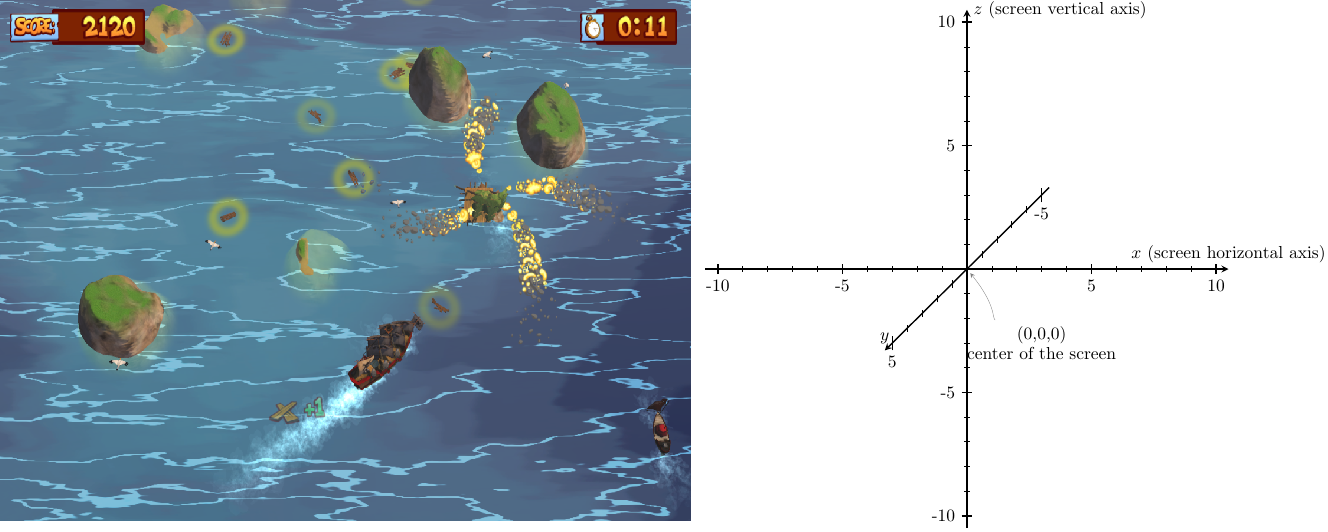
\includegraphics[width=130mm]{gameworld_coordinate.png}
\caption{3D Game World Coordinate \label{game_coordinate}}
\end{figure}
The game world is a never ending ocean which is shown on the screen such that players see everything what happened from the sky. Each object and event in the game are assigned with 3D location coordinates (\textit{x},\textit{y},\textit{z})(Figure \ref{game_coordinate}). An \textit{x} axis of this coordinate indicates horizontal axis of the screen. Zero \textit{x} axis is in the middle of the screen. Thus, an event happened on the right half of the screen will have positive \textit{x} value and an event happened on the left half of the screen will have negative \textit{x} value. \textit{y} axis indicates vertical axis in the game world which means -\textit{y} is a location under the ocean and +\textit{y} is above the ocean. \textit{z} axis indicates vertical axis of the screen. Zero \textit{z} axis is in the middle of the height of the screen, thus -\textit{z} is a location on the lower half of the screen and +\textit{z} is a location on the upper half of the screen. The visualization interface uses x coordinate information to represent body movement to the right or left and z axis to calculate screen speed as explained in the following sub section.

\subsection{Screen Speed}
In the game, a big number of positive events indicate a good player's performance. However, it is important to consider whether the events happened when the player's boat move fast or slowly \ref{t12}\ref{t14}. Getting all the bonuses while moving fast requires precise hand/body movement which indicates improvement in rehabilitation process. Boat speed while navigating the sea is basically the speed in which the screen scroll. This is calculated by identifying the location(apparition z coordinate $\theta_{apr}$) and time (apparition time $\textit{t}_{apr}$) of an object when it first appear on the screen, and location(event z coordinate $\theta_{evt}$) and time(event time $\textit{t}_{evt}$) when an event happened on that object. Screen speed($\upsilon_{scr}$) is distance between apparition location and event location divided by duration between apparition time and event time.

$$ \upsilon_{scr} = \frac{\theta_{evt}-\theta_{apr}}{\textit{t}_{evt}-\textit{t}_{apr}} $$

\section{Clustering}

In understanding the evolution of movements among different sessions over x-area, it is interesting to see what the common evolution of different section of the x-area\ref{t25}. The idea is to cluster similar distribution of movements (which is represented by events in the game) so that consecutive section which has similar evolution is represented by a single representation. This section explains how the clustering is done. First, a distance function used to calculate the difference between two consecutive section will be presented. Then, a clustering algorithm based on hierarchical clustering which incorporate this distance function will be explained.

\subsection{Distance Calculation}
Let S be a gameplay data set of $n_{ses}$ sessions. S is an ordered list of sections $s_i, 0 \le i < n_{sec}$. Each section contains events occurred on an x-axis unit among all sessions. More precisely, a  section $s_i$ is a sequence of triplets $s_i\lbrack j \rbrack, 0 \le j < n_{ses}$. Each triplet represents data set of a certain game session of a particular section $s_i$. The triplet consists of the number of negative, neutral and positive events. The profile of each section can be represented by a matrix of $n_{ses}$ x 3 dimensions. For instance, the following matrices represents a gameplay with 2 sessions and 3 sections:

\[
\textit{s}_1 = \begin{bmatrix}
  10 & 20 & 6\\
  20 & 5 & 18
\end{bmatrix}
\textit{s}_2 = \begin{bmatrix}
  20 & 40 & 10\\ 
  40 & 10 & 30
\end{bmatrix}
\textit{s}_3 = \begin{bmatrix}
  10 & 20 & 5\\
  16 & 4 & 12 
\end{bmatrix}
\]

In this example, we see that on the left part of the x-axis ($s_1$), the player got 10 negative, 20 neutral and 6 positive events for the first session. He then got 20 negative, 5 neutral and 18 positive events for the second session. On the middle part of the x-axis ($s_2$), on the first session he got 20 negative, 40 neutral and 10 positive events, while on the the second session he got 40 negative, 10 neutral, and 30 negative events.

Since the idea was to aggregate consecutive sections with similar movement pattern, a function to quantify the similarity between two sections is needed. In this case, we quantify the similarity by defining a distance function. Thus, distance equals 0 indicates that both sections are similar, while distance equals 1 indicates that both sections are different. We identified that there are two types of distance need to be considered: (i) how different both sections in term of event types proportion within each section (ii) how different both sections in term of the evolution of each event type throughout the sessions. For instance, with the (i) approach, $s_2$ and $s_3$ are similar, because triplets of each sessions are proportional ([20,40,10] is proportional to [10,20,5] and [40,10,30] is proportional to [16,4,12]). With the (ii) approach, $s_1$ and $s_2$ are similar, because the corresponding event types are proportional ([10,20] is proportional to [20,40], [20,5] is proportional to [40,10], and [6,18] is proportional to[10,30]).

Thus, for each pair of consecutive sequences ($\textit{s}_1$,$\textit{s}_2$) of \textit{S}, distance is defined as weighted sum of (i) and (ii), represented as $\textit{f}(\textit{s}_1,\textit{s}_2)$ and $\textit{g}(\textit{s}_1,\textit{s}_2)$ in the following formula:

$$d(\textit{s}_1,\textit{s}_2) = \alpha\textit{f}(\textit{s}_1,\textit{s}_2) + (1 - \alpha)\textit{g}(\textit{s}_1,\textit{s}_2)$$

Distance function $f(\textit{s}_1,\textit{s}_2)$ is based on a normalized euclidean distance between two triplets of the same session between two consecutive sections. The overall distance of both sections is the average euclidean distance of each triplets pair. To get a value of distance between 0 and 1, each Euclidean distance value is normalized by dividing it with maximum distance $\sqrt{3}$.

$$f(\textit{s}_1,\textit{s}_2) = \frac{\displaystyle\sum_{i=0}^{i < \lvert\textit{s}_1\lvert} \textit{N}ED(\textit{s}_1\lbrack i \rbrack,\textit{s}_2\lbrack i \rbrack)}{ \lvert\textit{s}_1\lvert}$$

$$ \textit{N}ED(\textit{s}_1\lbrack i \rbrack,\textit{s}_2\lbrack i \rbrack) = \frac{\sqrt{\displaystyle\sum_{j \in \{0,1,2\}}(\textit{s}_1'\lbrack i \rbrack\lbrack j \rbrack - \textit{s}_2'\lbrack i \rbrack\lbrack j \rbrack)^2}}{\sqrt{3}}$$

In this first distance function, $\textit{s}_1'$ and $\textit{s}_2'$ represent normalized value of $\textit{s}_1$ and $\textit{s}_2$. Since the first distance is to see the difference of event type proportion in each section, thus the values are normalized by the maximum value of each sessions in each section. In this case, two consecutive sections with different number of events but similar proportion of event type will have distance equals 0.  For example, the matrices presented previously can be normalized into the following matrices:

\[
s_1' = \begin{bmatrix}
  \frac{1}{2} & 1 & \frac{6}{20}\\ 
  1 & \frac{1}{4} & \frac{18}{20}
\end{bmatrix}
s_2' = \begin{bmatrix}
  \frac{1}{2} & 1 & \frac{1}{4}\\
  1 & \frac{1}{4} & \frac{3}{4} 
\end{bmatrix}
s_3' = \begin{bmatrix}
  \frac{1}{2} & 1 & \frac{1}{4}\\
  1 & \frac{1}{4} & \frac{3}{4} 
\end{bmatrix}
\]

Thus, distance \textit{f} of $s_1$ and $s_2$ equals 0.06, and distance \textit{f} of $s_2$ and $s_3$ equals 0.

The second distance function $\textit{g}(\textit{s}_1,\textit{s}_2)$ is based on a normalized euclidean distance between the same event type \textit{j} from different section. The overall distance of both sections is the average euclidean distance of each event type pair. For each event type distance, there are three different distance value defined: (i) if there are no events in both event type pairs, the distance is 0 (ii) if there is at least one event in one section and there are no events in the other section, the distance is 1 (iii) if both event type pairs has any events then the euclidean distance is calculated. Distance (i) and (ii) are defined to isolate empty regions. Thus when both sections are empty, it will be considered similar and will be clustered together. On the other hand, when only one section is empty while the other has some events, it will be considered as different session and therefore will not be clustered together. To get a value of distance between 0 and 1, each Euclidean distance value is then normalized by dividing it with maximum distance $\sqrt{\lvert\textit{s}_1\rvert}$.

$$\textit{g}(\textit{s}_1,\textit{s}_2) = \frac{\textit{g}_0(\textit{s}_1,\textit{s}_2) + \textit{g}_1(\textit{s}_1,\textit{s}_2) + \textit{g}_2(\textit{s}_1,\textit{s}_2)}{3}$$

\[\text{and for } j  \in \{0,1,2\}\text{, } g_j(\textit{s}_1,\textit{s}_2) = \left\{
  \begin{array}{ll}
    0 & \text{ if } \textit{s}_k\lbrack i \rbrack\lbrack j \rbrack=0 \text{ for each } 0 \leqslant j < |\textit{s}_k|\text{ and } \textit{k} \in \{1,2\}\\
    1 & \text{ if } \textit{s}_k\lbrack i \rbrack\lbrack j \rbrack=0 \text{ for each } 0 \leqslant j < |\textit{s}_k| \text{ and } \exists \textit{s}_p\lbrack i \rbrack\lbrack j \rbrack \neq 0,\\
      & k,p \in \{1,2\} \text{, } k \neq p\\
      & \\
	\multicolumn{2}{l}{\frac{\sqrt{\displaystyle\sum_{i=0}^{\lvert\textit{s}_1\lvert} (\textit{s}_1''\lbrack i \rbrack\lbrack j \rbrack - \textit{s}_2''\lbrack i \rbrack\lbrack j \rbrack)^2}}{\sqrt{\lvert\textit{s}_1\rvert}} \text{ otherwise}} 
  \end{array}
\right.
\]

Here, $s_1''$ and $s_2''$ represent normalized value of $s_1$ and $s_2$. In order to compare the evolution of the same event type between consecutive sections, the values are normalized by dividing it with maximum value of each event type in the section. Thus, the matrices presented previously can be normalized into the following:

\[
s_1'' = \begin{bmatrix}
  \frac{1}{2} & 1 & \frac{1}{3}\\ 
  1 & \frac{1}{4} & 1
\end{bmatrix}
s_2'' = \begin{bmatrix}
  \frac{1}{2} & 1 & \frac{1}{3}\\ 
  1 & \frac{1}{4} & 1
\end{bmatrix}
s_3'' = \begin{bmatrix}
  \frac{5}{8} & 1 & \frac{5}{12}\\
  1 & \frac{1}{5} & 1 
\end{bmatrix}
\]

Here, distance \textit{g} of $s_1$ and $s_2$ equals 0, and distance \textit{g} of $s_2$ and $s_3$ equals 0.06. 

\subsection{Clustering Algorithm}
The clustering algorithm follows Hierarchical Clustering algorithm \cite{maimon} which is a clustering analysis method used to build hierarchy of clusters. Overall, the clustering is done as follows: Initially, the data set is divided into sections the size of x-axis unit. Then, distance of consecutive sections are calculated. Two consecutive sections with distance below a specified threshold are then merged. This resulting in a new set of sections. Then, the distance of each consecutive sections of this new set of sections are calculated and again, if the new distance satisfies the threshold, the sections will be merged. This process is repeated until there is no distance falls below the threshold.







